
\section{Ontology Usage}

% ontologie mohou dobre popsat openstack architekturu, protoze openstack vyuziva message bus, service catalog. Ontologie slouzi pak nad ramec openstack sluzeb u serveru ale definuji i vlastni operacni systemy a pridruzene sluzby - monitorting, metering, firewally, backupy, log management atd

We started mapping the very

% ontologie je multitenantni podporuje vice reseni najednou

The Ontology can support many individual implementations at the time

% 

\subsection{Implementation details}

% Vytvorerin ontologie - protoege, na zaklade SOA ontologie
% testovani reasoningu pres pellet vyvozovani

Initial work on creating our Ontology was done in Protege, open-source ontology editor and framework for building intelligent systems.

The ontology is transformed into graph database using our python-bases service named django-ENC that can read and write ontology from OWL-DL XML files created by Protege and communicates with neo4j graph database through REST API. The graph databases are part of family of NoSQL databases and offer much better performance at any volume of data.

\begin{figure}[!h]
\centering
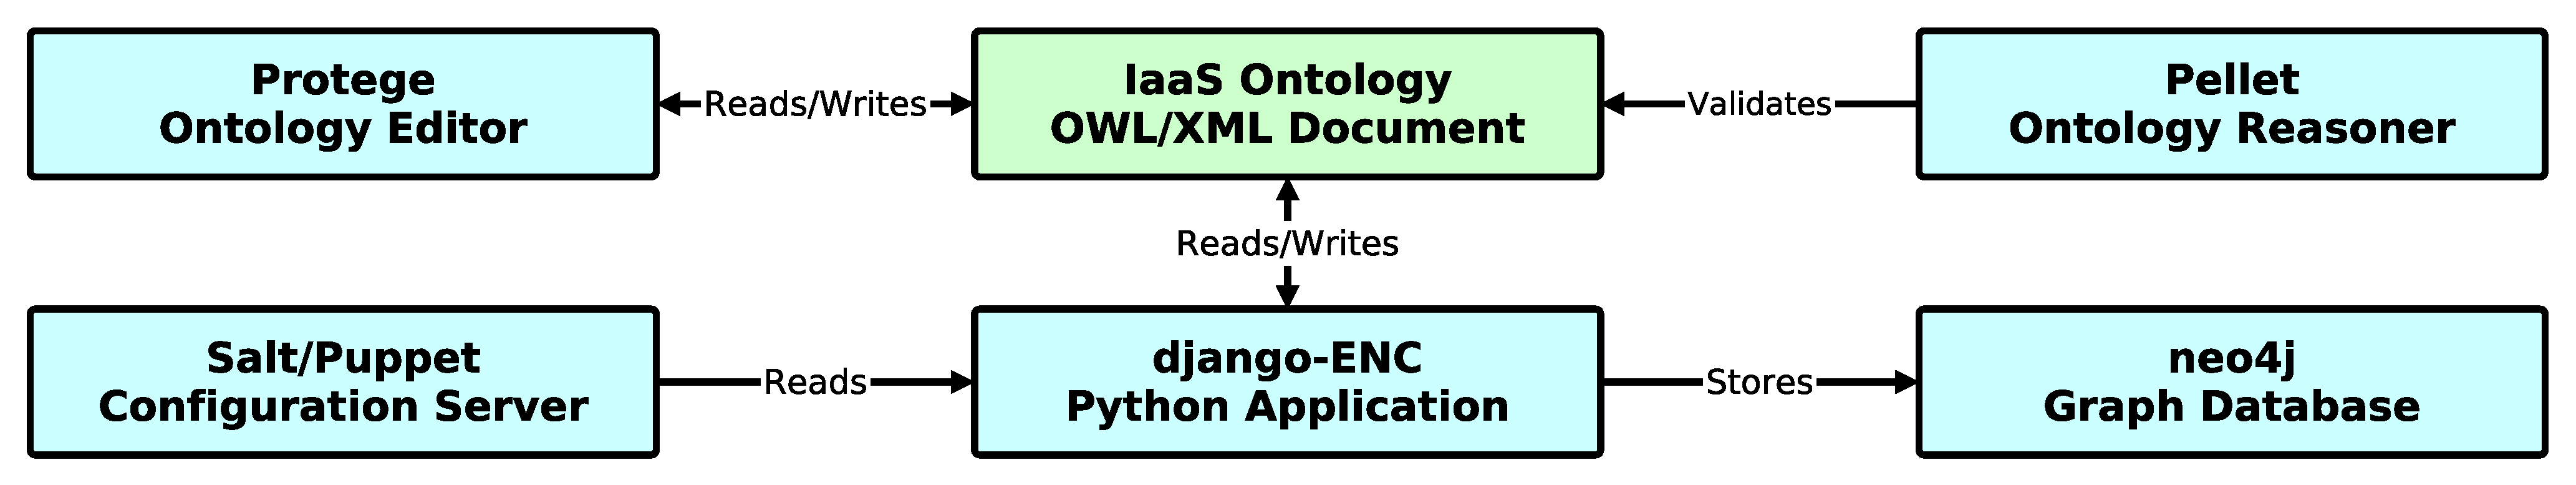
\includegraphics[scale=.17]{img/django_enc_arch.eps}
\caption{Ontology Service Architecture}
\label{fig:cm}
\end{figure}

The django-ENC service  use  web framework Django to deliver web services and asynchronous task queue Celery to perform time consuming tasks like ontology assertions and synchronizations between XML and graph database. Service expose it's owns HTTP REST API that can be consumed by configuration management tools like Salt or Puppet through their External Node Classification option.

The metada passed to CM tools is valid for 1st level of Cloud computing ontology [cite].

We have successfully tested service status enforcemet of several complete OpenStack installations by SaltStack configuration management tool with metadata acquired from Ontology ENC API.

The deployment process is not yet fully automated as there is need of setting up network and storage resources manually, but the progress in both configuration management tools and network and storage will allow better automation of these components by in-place agents or access protocols like SSH in the future.

\subsection{Samples of Ontology}

Given use case scenario Lab1 we have 3 virtual servers providing OpenStack and other core services in high-availability mode. These servers are virtualised in common. 20 physical servers  

\subsubsection{Service components of controller1}

Services located on controller server

\begin{lstlisting}
  <owl:Class rdf:about="#Glance">
    <owl:disjointWith>
      <owl:Class rdf:about="#"/>
    </owl:disjointWith>
    <owl:disjointWith>
      <owl:Class rdf:about="#ServiceInterface"/>
    </owl:disjointWith>
    <rdfs:subClassOf>
      <owl:Class rdf:about="#Composition"/>
    </rdfs:subClassOf>
  </owl:Class>
\end{lstlisting}

\subsubsection{Detail of service glance.image}

On of the services defined on the controller node is image service Glance. Following definitiong


\begin{lstlisting}
  <owl:Class rdf:about="#Glance">
    <owl:disjointWith>
      <owl:Class rdf:about="#"/>
    </owl:disjointWith>
    <owl:disjointWith>
      <owl:Class rdf:about="#ServiceInterface"/>
    </owl:disjointWith>
    <rdfs:subClassOf>
      <owl:Class rdf:about="#Composition"/>
    </rdfs:subClassOf>
    <owl:disjointWith>
      <owl:Class rdf:about="#ServiceInterface"/>
    </owl:disjointWith>
    <rdfs:subClassOf>
      <owl:Class rdf:about="#Composition"/>
    </rdfs:subClassOf>
  </owl:Class>
\end{lstlisting}

\subsubsection{Detail of data property type}

The resource can have data property and are derived mostly from Dublin Core metadata terms.

\begin{lstlisting}
  <owl:Class rdf:about="#Glance">
    <owl:disjointWith>
      <owl:Class rdf:about="#"/>
    </owl:disjointWith>
    <owl:disjointWith>
      <owl:Class rdf:about="#ServiceInterface"/>
    </owl:disjointWith>
    <rdfs:subClassOf>
      <owl:Class rdf:about="#Composition"/>
    </rdfs:subClassOf>
  </owl:Class>
\end{lstlisting}

\subsubsection{Detail of object property database}

Resources can have object property types that describe more complex relations. 

\begin{lstlisting}
  <owl:Class rdf:about="#Glance">
    <owl:disjointWith>
      <owl:Class rdf:about="#"/>
    </owl:disjointWith>
    <owl:disjointWith>
      <owl:Class rdf:about="#ServiceInterface"/>
    </owl:disjointWith>
  </owl:Class>
\end{lstlisting}
